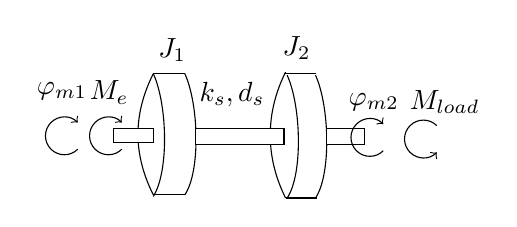
\begin{tikzpicture}[scale=2]


  \draw (1.14,-0.39) .. controls (1.01,-0.13) and (1.01,0.15) .. (1.14,0.41);


  \draw (0.5,-0.37) .. controls (0.6,-0.22) and (0.59,0.2) .. (0.5,0.4);

  \draw (0.3,-0.38) .. controls (0.4,-0.22) and (0.39,0.2) .. (0.3,0.4);

  \draw (1.33,-0.39) .. controls (1.43,-0.24) and (1.42,0.19) .. (1.33,0.39);

  \draw (1.15,-0.39) .. controls (1.25,-0.24) and (1.24,0.19) .. (1.15,0.39);

  \draw (0.3,-0.37) .. controls (0.17,-0.11) and (0.17,0.14) .. (0.3,0.4);

  \draw (0.3,0.40) -- (0.5,0.4);
  \draw (0.3,-0.37) -- (0.5,-0.37);
  \draw[fill=white] (0.05,-0.04) rectangle (0.3,0.05);

  \draw (0.57,-0.05) rectangle (1.13,0.05);

  \draw (1.13,0.4) -- (1.33,0.4);
  \draw (1.14,-0.39) -- (1.34,-0.39);
  \draw[fill=white] (0.57,-0.05) rectangle (1.13,0.05);
  \draw[fill=white] (1.4,-0.05) rectangle (1.64,0.05);


  \draw[->] (0.1,-0.08) arc[start angle=315, end angle=45, radius=0.12];
  \node at (0.02,0.28) {$M_e$};

  \draw[<-] (2.1,-0.1) arc[start angle=315, end angle=45, radius=0.12];
  \node at (2.15,0.22) {$M_{load}$};


  \draw[->] (-0.18,-0.08) arc[start angle=315, end angle=45, radius=0.12];

  \node at (-0.28,0.29) {$\varphi_{m1}$};


  \node at (1.7,0.22) {$\varphi_{m2}$};

  \node at (0.8,0.27) {$k_s,d_s$};

  \draw[->] (1.76,-0.09) arc[start angle=315, end angle=45, radius=0.12];

  \node at (0.42,0.55) {$J_1$};

  \node at (1.21,0.56) {$J_2$};


\end{tikzpicture}